\documentclass[10pt]{beamer}

\usepackage[utf8]{inputenc}
\usepackage{tcolorbox}
\usepackage{tikz}
\usetikzlibrary{intersections}
\usepackage{amsmath}


\tcbset{%
	basic/.style={colframe=black,
		      colback=white,
		      top= 0mm,
		      bottom = 2mm,
		      boxsep=0mm
		      }
}

    
\begin{document}  
    \beamertemplatenavigationsymbolsempty
    
    \frame{
	   \frametitle{Q1 Juillet 2015.}

	    Un point $P$ appartient à la diagonale $BD$ d'un carré $ABCD$. On note $c$ la longueur de chacun des côtés de ce carré. 
	    Démontrer l'égalité $$\overrightarrow{BP} \cdot \overrightarrow{DP} = ||\overrightarrow{AP}||^2 - c^2.$$

	    \vfill
	  
	  \pause
	  % hypothèses et thèse
	  \begin{tcolorbox}[basic] 
	      \begin{columns}[t]
		 
		 \column{.5\textwidth}\centering
		      
		      \underline{Hypothèses} 
		      \begin{itemize}
		      \item $ABCD$ carré.
		      \end{itemize}

		  
		  \column{.5\textwidth}\centering
		      
		      \underline{Thèse} \\
		      \smallskip
		      $\overrightarrow{BP} \cdot \overrightarrow{DP} = ||\overrightarrow{AP}||^2 - c^2.$
		
	      \end{columns}
	  \end{tcolorbox}
    
    
	   }

	   
 \frame{ % résolution ex1
	  \begin{columns}[t]
		\column{.5\textwidth}\centering 
		

			\underline{Dessin}\\
			
				  \begin{figure}[h]
				  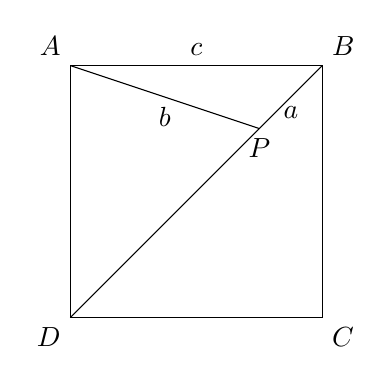
\begin{tikzpicture}[scale=0.8]
					\coordinate[label=above left:$A$] (A) at (-2,2);
					\coordinate[label=above right:$B$] (B) at (2,2);
					\coordinate[label=below right:$C$] (C) at (2,-2);
					\coordinate[label=below left:$D$] (D) at (-2,-2);
					\coordinate[label=below:$P$] (P) at (1,1);
					\draw (A) -- coordinate[label=above:$c$] () (B) -- (C) -- (D) -- cycle;
					\draw (A) -- coordinate[label=below:$b$] () (P);
					\draw (D) -- (P) -- coordinate[label=below:$a$] () (B);
%TODO dessin angle alpha					
				  \end{tikzpicture}
				  \end{figure}
			
				  \begin{tcolorbox}[basic] 
				      
				    \smallskip
				    \underline{Hypothèses} 
				    \begin{enumerate}
				    \item  $ABCD$ carré.
				    \end{enumerate}
							      
				    \underline{Thèse} \\
				    \medskip
				    $\overrightarrow{BP} \cdot \overrightarrow{DP} = ||\overrightarrow{AP}||^2 - c^2$.
				    \end{tcolorbox}
		
		
		\column{.5\textwidth}\centering
		
		\underline{Résolution}\\ \bigskip
		
		\begin{itemize}
		 \item $\overrightarrow{BP} \cdot \overrightarrow{DP} = -a(\sqrt{2}c-a)$,
		 \item $||\overrightarrow{AP}||^2 - c^2 = b^2 - c^2$.
		\end{itemize}

		
		\flushleft Thèse : $-a(\sqrt{2}c-a) = b^2 - c^2$.\\ \bigskip \medskip
		
		\begin{enumerate}
%TODO fraction +grand
		\item $\alpha = \frac{\pi}{4}$.
		\end{enumerate}
		
		\begin{itemize} 
		\item[$\heartsuit$]Pythagore généralisé.
		\end{itemize}
		
		$b^2 = a^2 + c^2 - \sqrt{2}ac$. \\
		\bigskip
		\medskip
%TODO aligner		
		$b^2 - c^2 = a^2 - \sqrt{2}ac = -a(\sqrt{2}c-a)$.
		
		
		\hfill $\qed$

   
	   \end{columns}
	   }
	  
  \frame{%Enoncé ex2
  
	\frametitle{Q2 Juillet 2015.}
	
	Soient $ABC$ un triangle rectangle en $A$, et $d$ une droite passant par
	$A$. On note $G$ la projection orthogonale de $B$ sur $d$, et $E$ la projection
	orthogonale de $C$ sur $d$. On note également $d_1$ la parallèle à $AC$ menée
	par $G$, et $d_2$ la parallèle à $AB$ menée par $E$. \bigskip
	\begin{itemize}
	 \item[$(a)$] Démontrer que les droites $d_1$ , $d_2$ et $BC$ sont concourantes.
	 \item[$(b)$] Déterminer le lieu géométrique du point d’intersection de $d_1$ et de
		      $d_2$ lorsque $d$ varie.
	\end{itemize}
	
	\vfill
	  
	  \pause	  
	  % Conditions
	  \begin{tcolorbox}[basic] 
	      	 
		      \medskip
		      \underline{Procédé} \\
		      \begin{itemize}
		       \item Repère orthonormé et équations cartésiennes,
		       \item[$(a)$] M.q. $d_1 ... d_2 = d_1 ... BC$,
		       \item[$(b)$] Point d'intersection en fonction de la pente de $d$.
		      \end{itemize}
		   		  	     
	  \end{tcolorbox}
	}
  \frame{%Résolution
	\begin{columns}[t]
		\column{.5\textwidth}\centering 
		

			\underline{Dessin}\\
%TODO continuer dessin			
				  \begin{figure}[h]
				  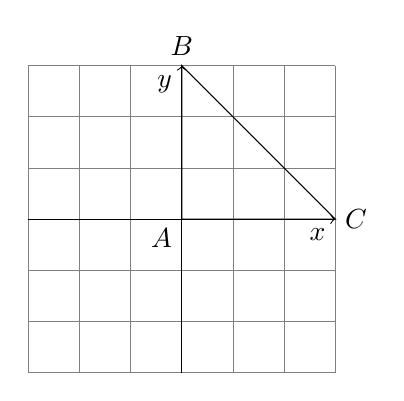
\begin{tikzpicture}[scale=0.65]
					\draw[help lines] (-3,-3) grid (3,3); 
					
					%AXES
					\draw[->] (0,-3) -- (0,3) coordinate[label=below left:$y$]();
					\draw[->] (-3,0) -- (3,0) coordinate[label=below left:$x$]();
					%TRIANGLE
					\coordinate[label=below left:$A$] (A) at (0,0);
					\coordinate[label=above:$B$] (B) at (0,3);
					\coordinate[label=right:$C$] (C) at (3,0); 
					\draw (A) -- (B) -- (C) -- cycle;
					

				
				  \end{tikzpicture}
				  \end{figure}
			\begin{tcolorbox}[basic]
			\smallskip
			\centering
			\underline{Procédé} \\
		        \smallskip
		        \begin{itemize}
		       \item Repère orthonormé et equations cartésiennes,
		       \item[$(a)$] M.q. $d_1 ... d_2 = d_1 ... BC$,
		       \item[$(b)$] Point d'intersection en fonction de la pente de $d$.
		      \end{itemize}
			\end{tcolorbox}
			
		\column{.5\textwidth}\flushleft
		      \underline{Résolution} \\
		      Soit un repère orthonormé $R=(O,X,Y)$ avec : \\
		      $A (0,0), B (0,b), C (c,0)$.	\\ \bigskip	          		      		      

%TODO symbole def et inter		      
		      \textit{Cas particulier : $d..x=0$} \\ \medskip 
		      $G=B$, $E=A$.\\
		      $d_1..d_2=B .. BC$. \\ \bigskip
%TODO agrandir frac
		      \textit{Cas général : $d..y=mx (m..R)$}  \\ \medskip 
		      $GB..y-b=\frac{-1}{m}x$ \\
%TODO symbol def et inter et agrandir frac		    
		      $G.. GB..d = (\frac{mb}{1+m^2},\frac{m^2b}{1+m^2})$ \\ 
		      $d_1 .. y = \frac{m^2b}{1+m^2}$. \\ \bigskip

%TODO symbol def et inter et agrandir frac
		      $EC..y=\frac{-1}{m}(x-c)$ \\
		      $E.. EC..d = (\frac{c}{1+m^2},\frac{mc}{1+m^2})$ \\
		      $d_2 .. x=\frac{c}{1+m^2}$. 
		      
	\end{columns}
  
	}
	
  \frame{ 
 %TODO symbol def et inter et agrandir frac et appartient et def		      	
	$d_1 .. d_2 = (\frac{c}{1+m^2},\frac{m^2b}{1+m^2}) .. BC .. \frac{x}{c} + \frac{y}{b} = 1. $ \hfill \qed (a) \\ \bigskip
%TODO symbol def et accolade et appartient a R et aggrandir frac
	Lieu .. .. $B (0,b)$ \\
		   $x= \frac{c}{1+m^2},$ \\
		   $y= \frac{m^2b}{1+m^2}$. \\
%TODO >=		   
	$x ..0,y > 0$ car $m..R$. \\
	$m^2=\frac{c}{x}-1$. \\
	Lieu .. $y = -\frac{b}{c}(x-c)$ et $x..[0,c[$. \hfill \qed (b)\\ \bigskip
%TODO dessin lieu 
	\centering
	
	\underline{Dessin}\\
%TODO continuer dessin			
				  \begin{figure}[h]
				  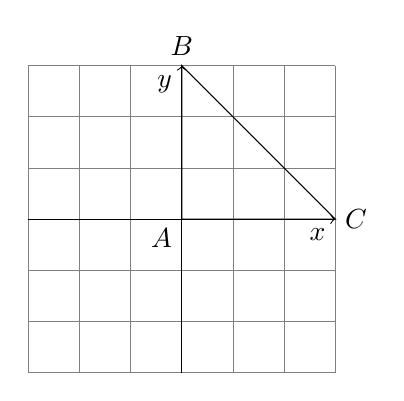
\begin{tikzpicture}[scale=0.65]
					\draw[help lines] (-3,-3) grid (3,3); 
					
					%AXES
					\draw[->] (0,-3) -- (0,3) coordinate[label=below left:$y$]();
					\draw[->] (-3,0) -- (3,0) coordinate[label=below left:$x$]();
					%TRIANGLE
					\coordinate[label=below left:$A$] (A) at (0,0);
					\coordinate[label=above:$B$] (B) at (0,3);
					\coordinate[label=right:$C$] (C) at (3,0); 
					\draw (A) -- (B) -- (C) -- cycle;
					

				
				  \end{tikzpicture}
				  \end{figure}
	
	
	}
\end{document}
